\section{Attribution Results}\label{sec:attribution}
% Budget 4.0 pages. Figs 5, 6, 7; Tables 3, 4.
\subsection{The Lone Trap}\label{sec:att-lone}
\begin{figure}[t]
\centering
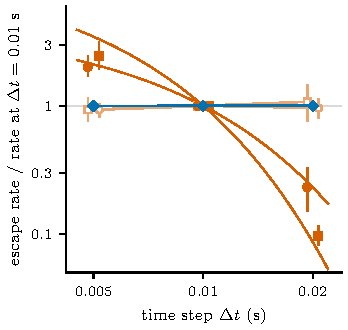
\includegraphics{../figures/fig5_dt.pdf}
\caption{Escape rate from deadlock snapshots against time step, normalised per snapshot by its value at $\Delta t=0.01$\,s (geometric means over snapshots with 95\% bootstrap intervals). Per-step noise is vermillion with filled circles ($\beta_{\rm ref}=1.5$) and squares ($2.5$) and its Arrhenius prediction from the exact discrete $k_BT_{\rm eff}$ as lines, $\sqrt{\Delta t}$-scaled noise light vermillion with open markers, and C3 RVO2 blue diamonds (inverse escape time).}
\label{fig:dt}
\end{figure}
\begin{figure}[t]
\centering
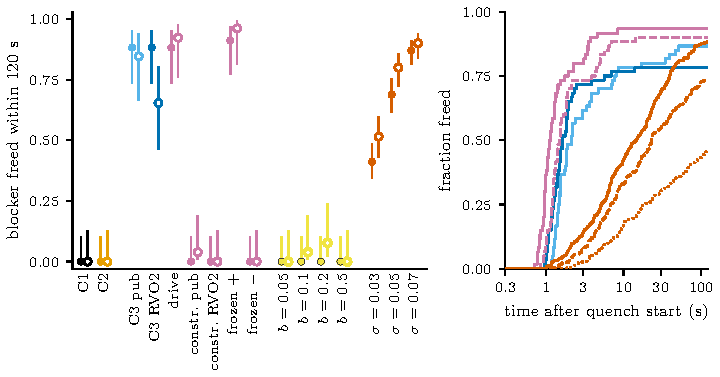
\includegraphics[width=\textwidth]{../figures/fig6_quench.pdf}
\caption{Left: fraction of lone-trap deadlock snapshots whose blocker is freed within 120\,s under each intervention, with Wilson 95\% intervals; right: Kaplan--Meier cumulative fraction freed against time for the arms that free, both strata pooled. Filled markers are lone-keystone snapshots and open markers those with a second trap; C1 is black, C2 orange, C3 published sky blue, C3 RVO2 blue, the ORCA drive, constraint and frozen-mean arms reddish purple, lateral bias yellow and noise vermillion, and on the right the drive-only arm is dashed, frozen mean $+$ solid, and noise $\sigma=0.03$, $0.05$, $0.07$\,m/s dotted, dashed and solid.}
\label{fig:quench}
\end{figure}
%
The quench library holds \EtwoNAll\ corrected-forward snapshots in two strata: all \EtwoNLK\ lone-keystone deadlocks and \EtwoNST\ drawn from the class with a second trap. The outcome is whether the blocker is freed within 120\,s (Fig.~\ref{fig:quench}); \pending{Table~3 (matched-control results for both classes) is input once the pair-class rows (E7b) exist}.

\paragraph{ORCA is its rest drive.}
At the lone keystone, C3 RVO2 frees \EtwoLKCThreeRVOFreed\ of \EtwoLKCThreeRVON\ blockers. ORCA's drive alone, with the constraint part removed, frees the same snapshots (discordant \EtwoLKDriveVsRVODiscA:\EtwoLKDriveVsRVODiscB), as does the published solver (drive only against it \EtwoLKDriveVsPubDiscA:\EtwoLKDriveVsPubDiscB); the constraint part alone frees \EtwoLKConstrRVOFreed. A constant goal-parallel push equal to the rest drive frees \EtwoLKFrozenPlusFreed\ blockers when it points to the door and \EtwoLKFrozenMinusFreed\ when it points away. C1 and C2 free none, and C2 reproduces C1 in \EtwoLemmaIdentical\ of \EtwoLemmaPairs\ paired runs, as Proposition~\ref{prop:rest} requires. Replays perturbed by $10^{-9}$\,m reproduce the C3 RVO2 outcome exactly (largest change in first-exit time \EtwoReplayCThreeRVOMaxDt\,s over \EtwoReplayN\ replays), and the snapshots it fails to free are those whose rest-state margin with ORCA's drive added stays positive (area under the ROC curve \EtwoLKMarginAUC). Every response is that of class L: ORCA frees the lone trap by adding a deterministic drive that removes the fixed point.

\paragraph{Matched noise acts differently.}
Per-step noise at $\sigma=0.07$\,m/s frees the lone keystone at the same rate, \EtwoLKNoiseCFreed\ of \EtwoLKNoiseCN\ runs (five seeds per snapshot) against \EtwoLKCThreeRVOFreed\ of \EtwoLKCThreeRVON. The match ends there. The snapshots that each arm leaves unresolved overlap with Jaccard index \EtwoLKJaccardC\ [\EtwoLKJaccardCLo, \EtwoLKJaccardCHi]. Replays disagree: over all \EtwoNAll\ snapshots the seeds split in \EtwoNoiseDisagreeC, with a within-snapshot standard deviation of the first exit time of \EtwoNoiseSDC\,s. Noise waits before it frees, with a Kaplan--Meier median time-to-free of \EtwoAllNoiseCMedianT\,s against \EtwoAllCThreeRVOMedianT\,s for C3 RVO2. The lateral bias, the deterministic control of class D, frees no lone keystone at any $b$ (upper Wilson bound \EtwoMaxBiasUpperLK), as expected when nothing is symmetric to break.

\paragraph{The time-step signature.}
The \EthreeN\ snapshots of the time-step test, spread over the collective barrier, test Eq.~\eqref{eq:ell} directly, with the noise set per snapshot so that $\beta_{\rm ref}=\Delta U/k_BT_{\rm eff}$ at $\Delta t=0.01$\,s is 1.5 or 2.5 (Fig.~\ref{fig:dt}). With per-step noise, $\ell=\ln\hat\lambda(0.005)/\hat\lambda(0.02)$ is \EthreeEllBA\ [\EthreeEllBALo, \EthreeEllBAHi] against a predicted \EthreeEllBAPred\ at $\beta_{\rm ref}=1.5$, and \EthreeEllBB\ [\EthreeEllBBLo, \EthreeEllBBHi] against \EthreeEllBBPred\ at $\beta_{\rm ref}=2.5$; the second falls short of the prediction, with an interval that excludes it. Over all \EthreeN\ snapshots the slope of observed on predicted $\ell$ through the origin is \EthreeSlope\ [\EthreeSlopeLo, \EthreeSlopeHi]. Scaling the noise with $\sqrt{\Delta t}$ removes the effect, $\ell=\EthreeEllScaled$ [\EthreeEllScaledLo, \EthreeEllScaledHi] (predicted \EthreeEllScaledPred). C3 RVO2 shows none: the log ratio of its escape times between the two steps is \EthreeCThreeLnRatio\ (largest magnitude \EthreeCThreeLnRatioMax), and it frees the same \EthreeCThreeFreed\ snapshots and holds the same \EthreeCThreeHeld\ at every step. Noise is thermal with the temperature of Eq.~\eqref{eq:teff}; ORCA is not thermal at all.

\paragraph{The second trap is pair-like.}
In the second-trap stratum full ORCA frees fewer blockers than its own drive, \EtwoSTCThreeRVOFreed\ against \EtwoSTDriveFreed\ of \EtwoSTCThreeRVON\ (discordant \EtwoSTDriveVsRVODiscA:\EtwoSTDriveVsRVODiscB, exact McNemar $p=\EtwoSTDriveVsRVOP$), so the constraint part works against the drive there. At restart it is negligible; it builds up once the agents start to move. In the held runs its door-ward component averages \StHeldConsMean\,N and reaches \StHeldConsMin\,N, cancelling on average a fraction \StHeldCancel\ of the drive, and it comes from the half-plane of a trapped neighbour abreast of the blocker. Geometry decides the outcome: C3 RVO2 frees \StPairFreed\ of \the\numexpr\StPairFreed+\StPairHeld\relax\ snapshots in which the blocker has exactly one trapped neighbour beside it at the jamb, against \StClusterFreed\ of \the\numexpr\StClusterFreed+\StClusterHeld\relax\ with two or more (Fisher $p=\StPairFisherP$). Where both free, C3 RVO2 is slower than its drive in \StPairedSlower\ of \StPairedN\ snapshots (median delay \StPairedDelay\,s; Kaplan--Meier medians \StTtfCThree\,s against \StTtfDrive\,s), through the neighbour's own ORCA response. This blocker--neighbour configuration is the pair geometry of Sect.~\ref{sec:pair}, and we return to it with the pair class in Sect.~\ref{sec:att-pair}.

\paragraph{Replay sensitivity of the published solver.}
Every deterministic arm, RVO2 ORCA included, reproduces its outcome exactly under the $10^{-9}$\,m replays. The published linear program does not: the outcome flips in \EtwoReplayCThreePubFlips\ of \EtwoReplayN\ replays, with first-exit times shifted by up to \EtwoReplayCThreePubMaxDt\,s, all at the second trap during slow creep. A replay of this size tests sensitivity, not randomness, so we read the flips as ill-conditioning of that implementation (class N for the published solver) and base every forward claim on RVO2.

\subsection{The Pair Class}\label{sec:att-pair}
\begin{figure}[t]
\centering
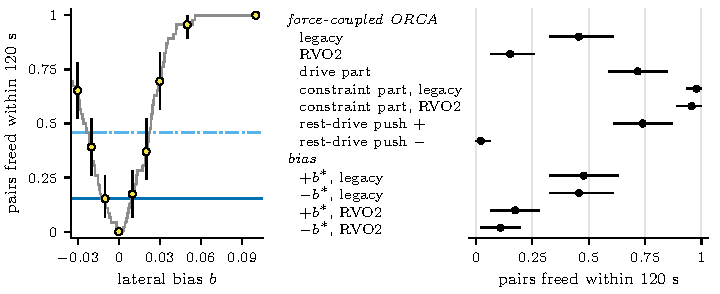
\includegraphics[width=\textwidth]{../figures/fig7_pair.pdf}
\caption{Left: fraction of the pair standoffs freed within 120\,s against the signed lateral bias $b$, with Wilson 95\% intervals, the static fold prediction as a step line and the C3 rates as horizontal lines; right: freed fraction per intervention. Lateral bias is yellow with the fold prediction in dark grey, C1 black, C2 orange, C3 published sky blue, C3 RVO2 blue, the ORCA drive, constraint and frozen-mean arms reddish purple, and noise vermillion.}
\label{fig:pair}
\end{figure}
%
The same probes applied to the \PairN\ standoffs of Sect.~\ref{sec:pair} give a different picture (Fig.~\ref{fig:pair}, right). C1 and C2 free none.

\paragraph{ORCA acts through its constraint part, and per implementation.}
The published solver frees \PairPubFreed\ standoffs and RVO2 \PairRvoFreed\ (discordant \PairPubRvoA:\PairPubRvoB, exact McNemar $p=\PairPubRvoP$), so at the pair every statement about ORCA is a statement about one solver. The constraint part alone frees \PairConsPubFreed\ (published) and \PairConsRvoFreed\ (RVO2), against none for C1: unlike at the lone trap, the half-planes act at the standoff, steering the members apart. The drive alone frees \PairDriveFreed, and a constant push equal to it frees \PairFrozenPlusFreed\ toward the door and \PairFrozenMinusFreed\ away from it. Yet full RVO2 ORCA frees fewer standoffs than its drive alone (discordant \PairDriveRvoA:\PairDriveRvoB, $p=\PairDriveRvoP$): together the two parts work against each other. This is the second-trap response of Sect.~\ref{sec:att-lone}, and the geometry is the same. In all \CtwsixN\ second-trap snapshots with exactly one trapped neighbour, that neighbour stands abreast on the other side of the axis, \CtwsixGapMin--\CtwsixGapMax\,m away surface to surface, as in the pair library; C3 RVO2 frees \CtwsixRvoFreed\ of them and its drive \CtwsixDriveFreed. Over 20\,s of C3 RVO2 the constraint part cancels on average \CtwsixCancel\ of the door-ward drive in the held second-trap runs and \PairTraceCancel\ in the held standoffs. A blocker with one trapped neighbour beside it is a pair standoff. Every deterministic arm reproduces its outcome in all \PairReplayN\ $10^{-9}$\,m replays.

\paragraph{One matched bias is not enough.}
The lateral bias is the class-D control. We matched it on rate alone, reading $b^\ast$ off the static fold curve so that it frees as many standoffs as C3, and then ran it on all \PairN\ standoffs at $\pm b^\ast$. Against the published solver, $b^\ast_{\rm pub}=\PairBstarPub$ frees \PairBsPubFreed\ against \PairPubFreed\ (discordant \PairBsPubA:\PairBsPubB, $p=\PairBsPubP$; with \PairN\ standoffs the 90\% interval of the rate difference, [\PairBsPubDiffLo, \PairBsPubDiffHi], is too wide to show equivalence within $\pm0.10$). Against RVO2, $b^\ast_{\rm RVO2}=\PairBstarRvo$ frees \PairBsRvoFreed\ against \PairRvoFreed\ (\PairBsRvoA:\PairBsRvoB, $p=\PairBsRvoP$). The held-out signatures separate the pairs. First, they free different standoffs: of the \PairBsPubEither\ that the published solver or its matched bias frees, both free \PairBsPubBoth\ (Jaccard \PairBsPubJac\ [\PairBsPubJacLo, \PairBsPubJacHi]), and the RVO2 match and RVO2 itself free disjoint sets (\PairBsRvoBoth\ of \PairBsRvoEither). Second, the bias has a handedness and ORCA has none: at $+b^\ast_{\rm pub}$ the favoured member exits first in \PairBsPubHand\ of \PairBsPubN\ freed standoffs; reversing the sign frees about as many (\PairBsPubMinusFreed), now with the other member first in all of them and largely a different set (discordant \PairBsPubRevA:\PairBsPubRevB); the published solver frees the lower member first in \PairPubLower\ of \PairPubFreed. Third, the bias acts on C1 through the fold, while ORCA succeeds only where its half-planes overcome its own drive. Both are deterministic, so the replay probe that exposed noise at the lone trap is silent here, and the class-D signatures do the separating. Noise frees almost every standoff even at its smallest amplitude (\PairNoiseLowFreed\ of \PairNoiseLowN\ runs at $\sigma=0.01$\,m/s), so it cannot be matched to either ORCA rate. At the pair, as at the lone trap, a control matched to ORCA's rate shares the headline number but not the mechanism.

\subsection{Revisiting the Conference Findings}\label{sec:att-conf}
\pending{Section 6.3 and Table~4 await E6/E6p (matched completion of whole runs), E7 (wall cells), E8/E9 (open geometries, initial-density sweep) and E11 (persistence-filtered overlaps).}
